\chapter{Kako složiti genomsku slagalicu od milion delova?}

\section{Šta je sekvenciranje genoma?}

Sa biološke strane, genom jednog organizma predstavlja njegov genetski materijal. Kod većine organizama, genetski materijal je sadržan u DNK. Kod čoveka, genom sadrži oko tri milijarde nukleotida. Genomi nekih organizama su i 100 puta veći od humanog genoma. 

Sa računarske strane, genom je niska karaktera nad azbukom $\{A, C, G, T\}$.

% nije mi jasan veliki razmak koji se napravi  u tekstu na ovom mestu xD

\subsection{Kratka istorija sekvenciranja genoma}

1977. godine Walter Gilbert i Frederick Sanger razvijaju nezavisne metode sa sekvenciranje DNK, za koje su, 1098. godine, podelili su Nobelovu nagradu.
Njihove metode za sekvenciranje su bile veoma skupe - 3 milijarde dolara za sekvenciranje humanog genoma.
\\
\\
Krajem 2000-tih Sanger metodom je sekvencioniran veliki broj genoma. Visoka cena je bila ograničavajući faktor i za dalji napredak je bila neophodna nova tehnologija sekvencioniranja.
\\
\\
\textbf{NGS} predstavlja metode nove generacije sekvencioniranja. Krajem 2000-tih, na tržištu se pojavljuju nove mašine za sekvenciranje. \textit{Illumina} smanjuje trošak sekvencioniranja humanog gemona sa 3 milijarde na 10 hiljada dolara. Kompanija \textit{Complete Genomics} otvara genomsku fabriku u Silikonskoj dolini koja sekvencionira stotine genoma mesečno.
Pekinški genomski institut (BGI - Beijing Genome Institute) preuzima Complete Genomics 2013. godine i postaje najveći svetski centar za sekvenciranje genoma.
Na slici \ref{slika:cena} prikazano je kako se cena sekvencioniranja menjala godinama.


\begin{figure}[H]
	\centering
	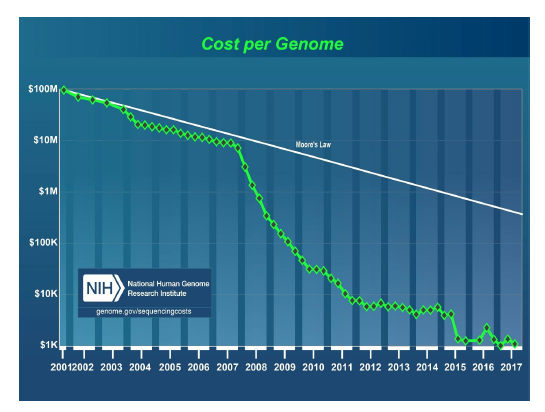
\includegraphics[width=1\textwidth]{poglavlja/3/slike/cena_sekvencioniranja.png}
	\caption{Cena sekvencioniranja kroz istoriju.}
	\label{slika:cena}
\end{figure} 



\subsection{Sekvenciranje ličnih genoma}

Genomi se kod različitih ljudi razlikuju na malom broju pozicija (u proseku sadrže jednu mutaciju na hiljadu nukleotida). Ova razlika je odgovorna za različite visine kod ljudi, da li će imati sklonost ka visokom holesterolu ili ne, za veliki broj genetskih bolesti, itd.
\\
\\
2010: Nicholas Volker je postao prvo ljudsko biće čiji je život spašen zahvaljujući genomskom sekvencioniranju.
Lekari nisu mogli da postave tačnu dijagnozu i morali su da ga podvrgnu velikom broju operacija pokušavajući da je utvrde. Sekvenciranje je otkrilo retku mutaciju na jednom genu (XIAP) koja je bila povezana sa oštećenjem njegovog imunog sistema. Ovo otkriće je navelo lekare na adekvatnu terapiju koja je rešila problem.

\section{Eksplozija u štampariji}

Zamislite da imamo hiljadu kopija istog izdanja novina na jednoj gomili, a ispod njih postavljen je dinamit. Upalimo fitilj i zamislimo da nije sve samo izgorelo već da se raspršilo u milione delića papira. Kako možemo da iskoristimo te deliće da bismo saznali koje su bile vesti iz tog izdanja? Ovaj problem nazvaćemo \textbf{Problem novina} (\ref{slika:eksplozija}). 

\begin{figure}[H]
	\centering
	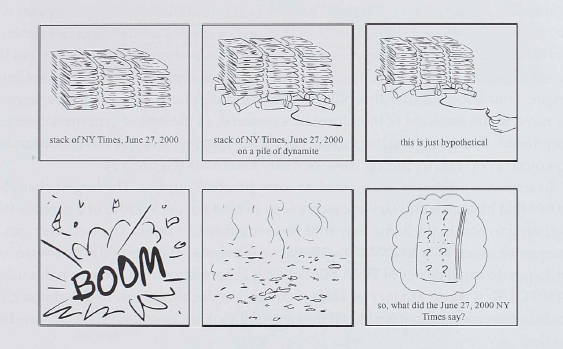
\includegraphics[width=1\textwidth]{poglavlja/3/slike/eksplozija.png}
	\caption{Problem novina poslužiće nam u razumevalju problema slaganja genoma.}
	\label{slika:eksplozija}
\end{figure} 


Problem novina je mnogo teži nego što izgleda. Kako smo imali više kopija istog izdanja, i kako smo izgubili neki deo informacija prilikom eksplozije, ne možemo samo da prilepimo deliće novina kao da su slagalica. Umesto toga, potrebno je da preklopimo delove različitih novina kako bismo rekonstruisali jedan primerak.


\begin{figure}[H]
	\centering
	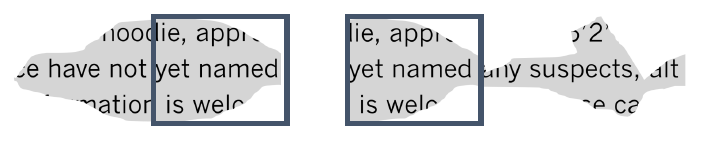
\includegraphics[width=1\textwidth]{poglavlja/3/slike/delici.png}
	\caption{Spajanje delova različitih novina koji se jednim delom preklapaju.}
	\label{slika:delici}
\end{figure} 


Kakve sad to veze ima sa našim problemom? Određivanje redosleda nukleotida u genomu, odnosno sekvenciranje genoma, predstavlja bitan problem u bioinformatici. Dužine genoma variraju: humani genom je dugačak oko 3 milijarde nukleotida, dok je genom jendoćelijskog organizma Amoeba dubia čak 200 puta duži. 


Moderne mašine za sekvenciranje (sekvenceri) ne mogu da pročitaju ceo genom nukleotid po nukleotid od početka do kraja (kao što bismo pročitali knjigu).
Mogu samo da iseckaju genom i generišu njegova kratka očitavanja. Kako to zapravo funkcioniše (\ref{slika:sekvenciranje})? Sekvencer dobija milione kopija istog genoma. Zatim vrši očitavanja čime dobijamo deliće odnosno kratke podniske. Neki delovi odnosno očitavanja biće izgubljena (kao delići novina u eksploziji, dakle gubimo deo informacija). Očitavanja su izmešana i ono što nam sekvencer daje je zapravo kolekcija podniski koje treba spojiti u jednu. Sastavljanje genoma nije isto kao i slaganje slagalice: moramo da koristimo preklapajuća očitavanja da bismo rekonstruisali genom.


\begin{figure}[H]
	\centering
	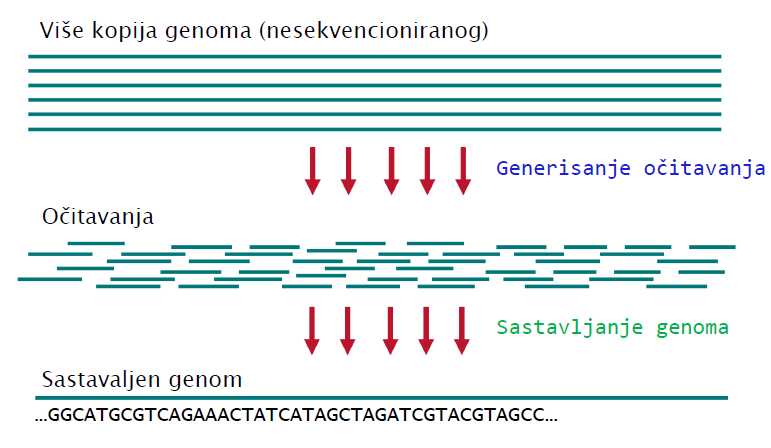
\includegraphics[width=1\textwidth]{poglavlja/3/slike/sekvencioniranje.png}
	\caption{Ilustracija problema.}
	\label{slika:sekvenciranje}
\end{figure} 


\section{Problem sekvenciranja genoma}

\begin{problem}
	[Problem sekvencioniranja genoma] Rekonstruisati genom na osnovu očitavanja.
	\\ Ulaz. Kolekcija niski Reads.
	\\ Izlaz. Niska Genome rekonstruisana na osnovu Reads.
\end{problem}

% ovo dopuniti sa snimka pošto nema ni u knjizi baš
Ovo nije dobro definisan problem. 


\subsection{k-gramski sastav niske}

k-gramski sastav niske $Text$ ($Composition_k(Text)$) predstavlja kolekcija podnsiki dužine $k$ niske $Text$, uključujući duplikate. Na primer:


% ovo sigurno može lepše xD (slajd 32)
\begin{align*}
	Composition_3(TAATGCCATGGGATGTT) =& \\
	TAA AAT ATG TGC GCC CCA CAT ATG TGG GGG GGA GAT ATG TGT GTT =& \\
	AAT ATG ATG ATG CAT CCA GAT GCC GGA GGG GTT TAA TGC TGG TGT
\end{align*}

Sada možemo malo bolje da definišemo problem.

\begin{problem}
	[Problem rekonstrukcije niske] Rekonstruisati nisku na osnovu njenog k-gramskog sastava.
	\\ Ulaz. Kolekcija k-grama.
	\\ Izlaz. Niska Genome takva da je $Composition_k(Genome)$ ekvivalentno kolekciji k-grama
\end{problem}


Naivni pristup ovom problemu bio bi da odaberemo jedan k-gram za početni. Zatim nižemo ostale tako da se sufiks poslednjeg odabranog poklopi sa prefiksom nekog od preostalih k-grama. Pri tome, ako ima više takvih k-grama, biramo jedan, bilo koji, Na ovaj način možemo doći do rešenja, ali je veoma skupo. Pri tome, velika je šansa da ćemo se negde zaglaviti (tj. nijedan od preostalih k-grama neće biti kandidat za nadovezivanje na tekuću nisku) ili zbog izbora početnog k-grama ili zbog izbora nekog od preostalih k-grama kada je postojalo više odgovarajućih. Sledeći primer ilustruje ovaj problem:

Neka nam je dat sledeći 3-gramski sastav: 
$$AAT ATG ATG ATG CAT CCA GAT GCC GGA GGG GTT TAA TGC TGG TGT$$

Treba rekonstruisati nisku koja ima takav sastav. Biramo početni 3-gram, neka to bude na primer $TAA$. Zatim na njega treba nadovezati 3-gram koji počinje njegovim sufiksom dužine 2, odnosno onaj 3-gram koji ima prefiks $AA$. U našem slučaju, postoji jedan takav 3-gram i njega nadovezujemo na tekuću nisku, tako da sada imamo $TAAT$. Zatim biramo 3-gram čiji je prefiks $AT$. Ovog puta imamo 3 kandidata, ali, na našu sreću, sva tri su isti 3-grami, $ATG$. U takvom slučaju nije bitno koji smo odabrali, jer su svi jednaki. Nadovezujemo ga na tekuću nisku i dobijamo $TAATG$. Tražimo 3-grame sa prefiksom $TG$, koji do sad nisu upotrebljeni. Ponovo pronalazimo 3 kandidata. Međutim, u ovom slučaju, svi kandidati predstavljaju različite 3-grame, a to su $TGC$, $TGG$ i $TGT$. Naivni pristup kaže da biramo jedan od njih, i recimo da smo odabrali $TGT$ i dobili nisku $TAATGT$. Sada nam je potrebam 3-gram sa prefiksom $GT$ i tu dolazi do zaglavljivanja! 
Imamo još 3-grama koji nisu iskorišćeni za rekonstrukciju niske, ali nijedan ne možemo da iskoristimo u ovom trenutku! U takvim situacijama treba se vratiti u nazad do koraka u kom je bilo više kandidata.


\section{Rekonstrukcija niske kao problem Hamiltonove putanje}

Videli smo da nam naivni pristup ne odgovara i moramo smisliti bolje rešenje. Mogli bismo da iskoristimo znanja iz teorije grafova za rešavanje ovakvog problema. U tom slučaju, prvi zadatak je da našu nisku predstavimo u vidu grafa.


\subsection{Genom kao putanja}

Vratimo se na prethodni primer. Dat nam je k-gramski sastav niske :
$$Composition_3(TAATGCCATGGGATGTT) =$$
$$ TAA AAT ATG TGC GCC CCA CAT ATG TGG GGG GGA GAT ATG TGT GTT$$

Njega treba predstaviti kao graf. Možemo da napravimo po jedan čvor za svaki od k-grama. Zatim, potrebne su nam grane koje će povezati te čvorove. Dvs čvora su povezana usmerenom granom ako izlazni čvor ima sufiks jednak prefiksu ulaznog čvora te grane, kao što je prikazano na slici \ref{slika:graf1}.

\begin{figure}[H]
	\centering
	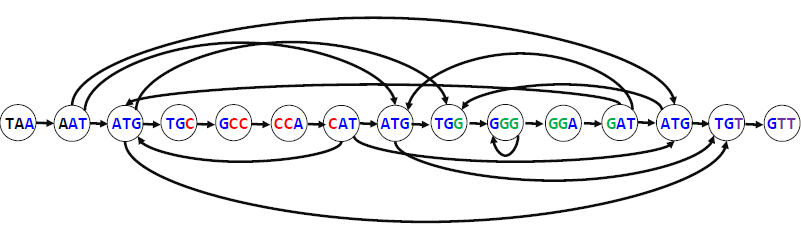
\includegraphics[width=1\textwidth]{poglavlja/3/slike/graf1.png}
	\caption{Graf koji odgovara k-gramskom sastavu niske $TAATGCCATGGGATGTT$.}
	\label{slika:graf1}
\end{figure} 

Jasno je da postoji više puteva u ovom grafu. Postavlja se pitanje, da li možemo da pronađemo genomsku putanju u ovom grafu, od svih koje postoje?

Podsetimo se šta je Hamiltonova putanja. Hamiltonova putanja je putanja koja posećuje svaki čvor u grafu tačno jednom. To je upravo ono što nam je potrebno za rešavanje problema. Svaki čvor predstavlja jedan k-gram i porebno nam je da svi k-grami budu uključeni u rekonstruisanu nisku tačno jednom.

\begin{problem}
	[Problem Hamiltonove putanje]
	Naći Hamiltonovu putanju u grafu.
	\\ Ulaz. Graf.
	\\Izlaz. Putanja koja posećuje svaki čvor u grafu tačno jednom.
\end{problem}

Iako deluje kao da smo rešili sve probleme, zapravo smo naišli na još jednu veliku prepreku. Naime, pronalaženje Hamiltonovog puta u grafu je NP-kompletan problem, što znači da ne postoji efikasan algoritam koji to radi.

U tom slučaju, moramo da se vratimo na početak, a to je predstavljanje k-gramskog sastava grafom.


\section{Rekonstrukcija niske kao Ojlerove putanje}

Mogu da se obeležavaju 3-grami kao čvorovi ili 3-grami kao grane. Kako obeležavamo početni i krajnji čvor grane?
za granu TAA- Prefiks $TA\rightarrow AA$ Sufiks. Dakle 3-grami su grane a 2-grami su čvorovi.

%% Sada ide animacija o lepljenju identično obeleženih čvorova

\subsection{Problem Ojlerove putanje}

\begin{problem}[Problem Ojlerove putanje]
	~\\ Pronaći Ojlerovu putanju u grafu.
	\\ Ulaz. Graf.
	\\ Izlaz. Putanja koja posećuje svaku granu u grafu tačno jednom.
\end{problem}

\section{De Brojnovi grafovi}

Konstruisali smo de Brojnov grav na osnovu genoma, ali u realnim primenama, genom je nepoznat.


%% ide animacija o konstrukciji de brojnovog grafa kad je genom nepoznat

De Brojnov graf na osnovu kolekcije k-grama.
Svaka grana je označena jednim k-gramom. Svaki čvor je označen prefiksom/sufiksom izlazne/ulazne grane. Zalepljeni su svi čvorovi sa identičnim oznakama.

\begin{problem}[Problem Ojlerovog ciklusa]
	~\\ Pronaći ciklus Ojlerovom grafu.
	\\ Ulaz. Graf.
	\\ Izlaz. Ciklus koja posećuje svaku granu tačno jednom.
\end{problem}

\begin{teorema}[Ojlerova teorema]
	Svaki povezan graf i balansiran graf je Ojlerov.
\end{teorema}

Kažemo da je graf povezan ako za ma koja dva čvora postoji putanja koja ih povezuje.


%% MRAVI DOKAZUJU OJLEROVU TEOREMU

\begin{verbatim}
EulerianCycle(BalancedGraph)
form a Cycle by randomly walking in BalancedGraph (avoiding already visited edges)
while Cycle is not Eulerian
select a node newStart in Cycle with still unexplored outgoing edges
form a Cycle' by traversing Cycle from newStart and randomly walking afterwards
Cycle \leftarrow Cycle'
return Cycle
\end{verbatim}

\section{Sastavljanje parova očitavanja}

Od očitavanja do de Brojnovog grafa do genoma može se javiti više Ojlerovih putanja u grafu.

\subsection{DNK sekvenciranje sa parovima očitavanja} 

Imamo više identičnih kopija genoma i na slučajnim pozicijama sečemo genom na fragmente iste dužine \textit{InsertLength}. Zatim generišemo parove očitavanja: dva očitavanja sa krajeva svakog fragmenta na fiksiranoj udaljenosti.
Pod uparenim k-gramom podrazumevamo par k-grama na fiksiranom rastojanju d u genomu. Na primer, TCA i TCC na rastojanju d=11 čine jedan upareni k-gram.

\begin{problem} [Problem rekonstrukcije niske na osnovu parova očitavanja]
	~\\ Rekontruisati nisku na osnovu njenih uparenih k-grama.
	\\ Ulaz. Kolekcija uparenih k-grama.
	\\ Izlaz. Niska Text takva da je PairedComposition(Text) jednak kolekciji uparenih k-grama. 
\end{problem}

Kako konstruisati upareni de Brojnov graf na osnovu uparenog k-gramskog sastava?
Pretpostavimo da je dat genom (niska Genome). Posmatrajmo genom kao putanju u grafu obeleženom na osnovu njegovog uparenog kgramskog sastava.
\\
Pretpostavili smo da je dat genom (niska Genome). Posmatrali smo genom kao putanju u grafu obeleženom na osnovu njegovog uparenog k-gramskog sastava
\\
Sada pretpostavimo da nije dat genom već samo upareni k-gramski sastav

%% animacije, SVUDA ANIMACIJE!!!!!

~\\ Upareni de Brojnov graf na osnovu kolekcije uparenih k-grama:
\\ – Svaka grana je označena jednim uparenim k-gramom
\\ – Svaki čvor je označen prefiksima/sufiksima izlazne/ulazne grane
\\ – Zalepljeni su svi čvorovi sa identičnim oznakama.

\section{U realnosti}

Ovde smo imali neke nerealne pretpostavke.
\begin{itemize}
	\item  Savršena pokrivenost genoma očitavanjima (svaki k-gram iz genoma je očitan)
	\item Očitavanja ne sadrže greške
	\item Rastojanja između očitavanja u okviru parova očitavanja su egzaktna
	\item Nesavršena pokrivenost genoma očitavanjima (svaki k-gram iz genoma je očitan)
	\\ Očitavanja ne sadrže greške
	\\ Rastojanja između očitavanja u okviru parova očitavanja nisu egzaktna
\end{itemize}

\subsection{Savršena pokrivenost}

Prva nerealna pretpostavka je savršena pokrivenost.
\\
Očitavanja dužine 250 nukleotida dobijena Illumina tehnologijom predstavljaju samo mali deo 250-grama unutar genoma.
\\
Rešenje: razbiti dobijena očitavanja na kraće k-grame
\\
\\
Druga nerealna pretpostavka: očitavanja ne sadrže greške.

\newpage
\section{Zadaci sa vežbi}
U nastavku će biti predstavljeni zadaci sa vežbi na kursu rađeni u programskom jeziku Python.


